\chapter{Future Work}
FEMCARE is a working screening and awareness platform, but several limitations described in Chapter 3 point to clear next steps. The planned extensions are described in this chapter.

\section{Multimodal AI Health Assistant}

The current assistant accepts text input only. A planned extension is a multimodal assistant that accepts text, voice, and images, and answers within the same women's reproductive health scope.

\begin{itemize}
    \item \textbf{Voice Input and Output:} Speech-to-text would let users describe symptoms by speaking, and text-to-speech would read responses aloud. Support for Gujarati and Hindi is a priority given the intended user base in Vadodara.
    \item \textbf{Image Input:} Users could upload a photo of a skin concern such as acne or dark patches, or a photo of a lab report. Lab report images would be read using OCR to fill the LH and FSH fields automatically instead of manual entry. In the longer term, a dedicated model for ovarian ultrasound images could support the risk assessment.
    \item \textbf{Unified Pipeline:} Every input type would be converted to a common representation and passed through the existing scope check, urgency check, and user-context enrichment before the LLM is called, so the topic restriction and safety behaviour remain unchanged.
\end{itemize}

Image and voice data are more sensitive than typed answers. This extension would therefore require explicit user consent, storage protected by the same Row Level Security policies, and a clear statement that all outputs are informational and not a diagnosis.

\section{Clinical Validation and Model Improvement}

The PCOS classifier has not been independently clinically validated (Section 3.7). Future work includes testing on larger and more diverse datasets, collecting clinician-verified labels, and reporting standard metrics such as precision, recall, and AUC. Data from Indian populations would also address the generalisation concern raised in the literature survey.

\section{Explainable Predictions}

Users currently see a risk level and a confidence percentage but not the reasons behind them. Adding feature-level explanations, for example using SHAP \cite{lundberg2017}, would show which inputs contributed most to a result. This addresses the trust and explainability gap identified in Section 2.4.

\section{Privacy-Preserving Learning}

Federated learning or on-device processing could allow the model to improve over time without centralising sensitive health data. This would build on the privacy-focused approaches discussed in the literature survey.

\section{Provider and Telemedicine Features}

The Find Care module currently uses a fixed list of ten providers in Vadodara, and changing it requires a source code change. Planned improvements include:

\begin{itemize}
    \item \textbf{Admin Interface:} A dashboard for adding and editing provider details, with provider data stored in the database instead of the source code.
    \item \textbf{Provider Availability:} Working hours and days off defined by each provider, replacing the fixed sixteen daily slots.
    \item \textbf{Wider Coverage:} Providers from cities beyond Vadodara.
    \item \textbf{Video Consultation:} Online appointments through video calls, extending the platform into telemedicine, which is outside the current scope.
\end{itemize}



\chapter{Research Paper and Plagiarism Report}
\section{Paper}

\subsection*{Research Paper Introduction}

The research paper titled \textbf{``FemCare: An XGBoost-Based Platform for PCOS Risk Assessment and Menstrual Cycle Length Prediction''} presents an AI-based women's healthcare platform developed for menstrual cycle management and PCOS risk assessment. The study uses two XGBoost models: a classification model for PCOS risk assessment and a regression model for predicting menstrual cycle length. The paper also discusses menstrual tracking, mood monitoring, and gynecologist appointment support. The proposed system is designed as a decision-support tool and is not intended to replace professional medical diagnosis.

\subsection*{Research Paper Details}

\begin{itemize}
    \item \textbf{Title:} FemCare: An XGBoost-Based Platform for PCOS Risk Assessment and Menstrual Cycle Length Prediction
    
    \item \textbf{Authors:} Dhvani Milin Chokshi, Kashish Mayur Shah, Krusha Maheshbhai Paghadal, Siddhi Chiragbhai Upadhyay
    
    \item \textbf{Affiliation:} Department of Computer Science and Engineering, Parul Institute of Engineering and Technology, Parul University, Vadodara, Gujarat, India
    
    \item \textbf{Research Area:} Artificial Intelligence, Machine Learning, Women's Healthcare
    
    \item \textbf{Primary Techniques:} XGBoost Classification and XGBoost Regression
    
    \item \textbf{Paper Length:} 9 pages
    
    \item \textbf{Publication Status:} Research paper prepared for academic/research submission
\end{itemize}

\subsection*{Abstract}

FemCare is a women's healthcare platform built for menstrual cycle management and PCOS risk assessment. It uses two XGBoost models, one for PCOS risk classification and another for predicting the length of the next menstrual cycle. The study reports 99.85\% accuracy for PCOS prediction and a mean absolute error of 1.89 days for cycle-length prediction. In addition to prediction, the platform supports period and mood tracking and gynecologist appointment assistance. The system is intended as a decision-support tool rather than a diagnostic system.

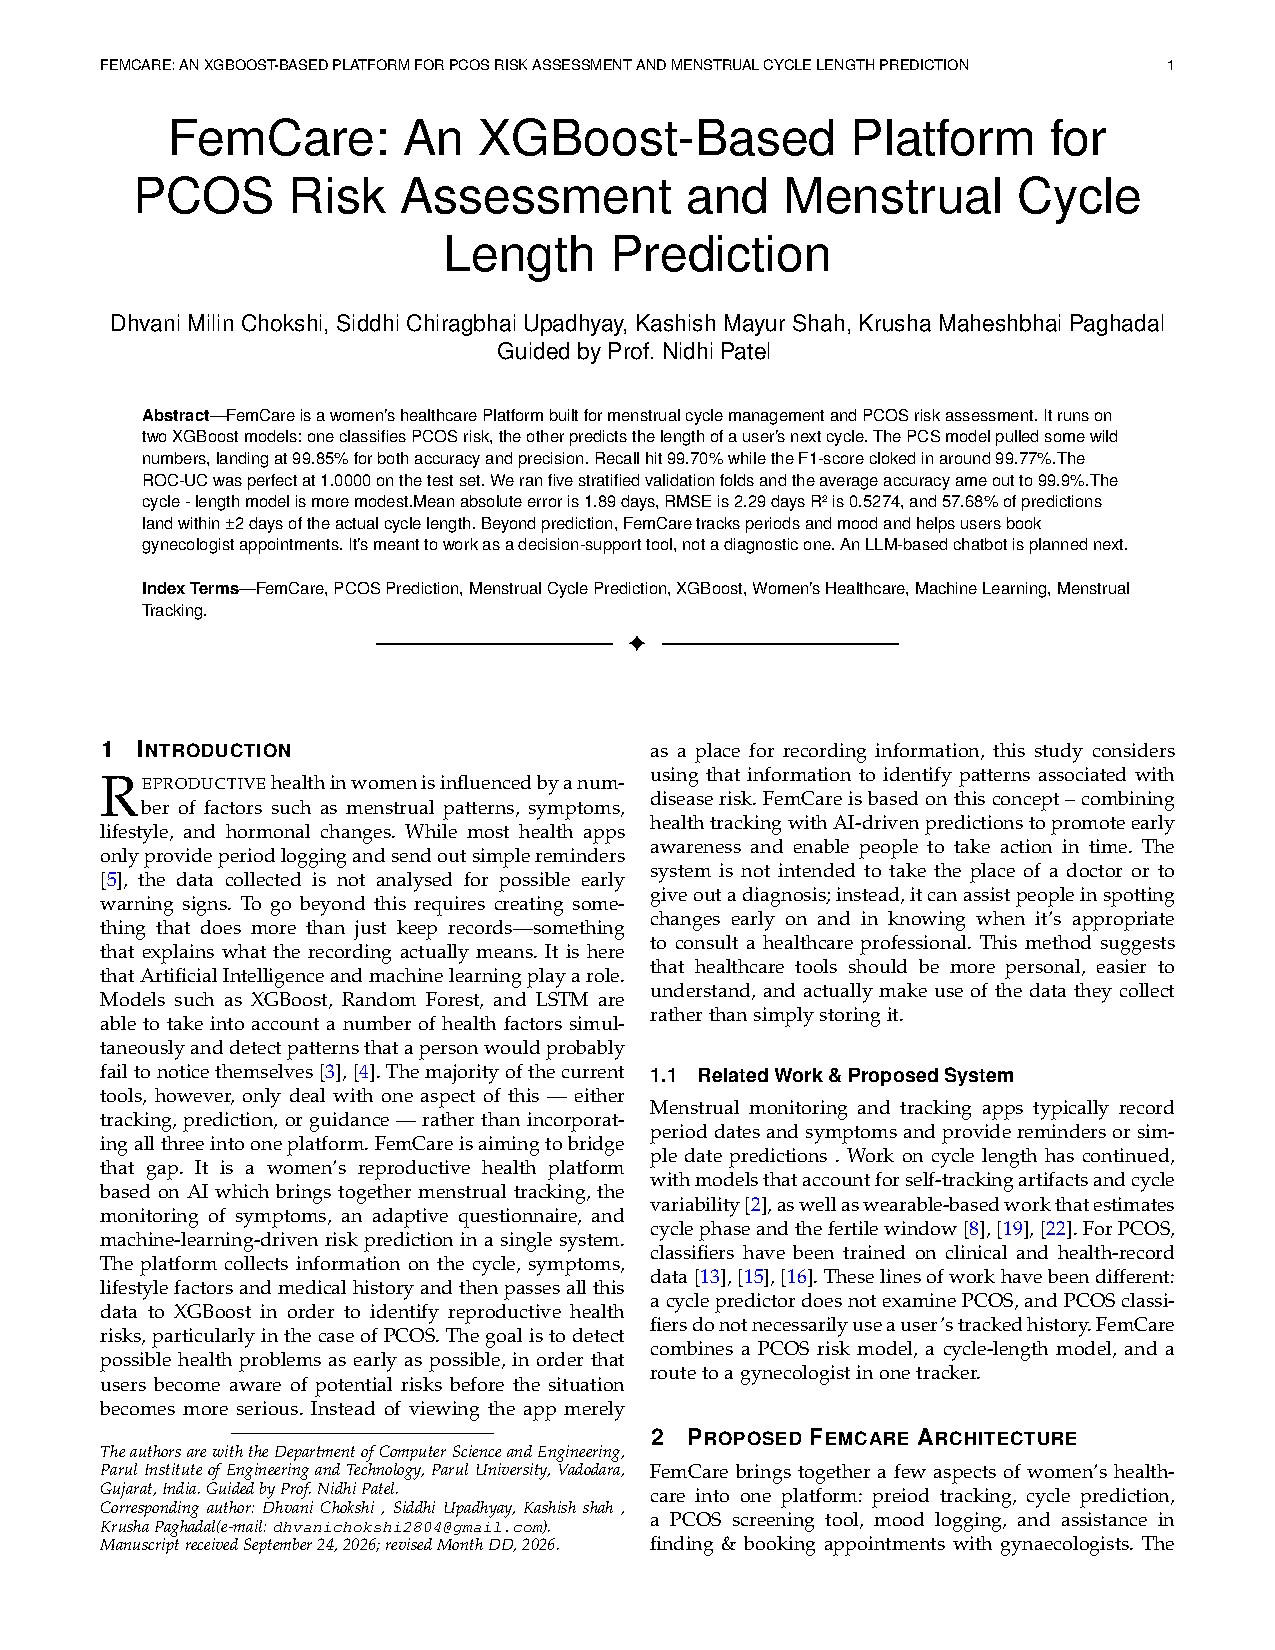
\includepdf[
    pages=-,
    fitpaper=true
]{ResearchPaper.pdf}

\section{Plagiarism and AI detection report paper}

\subsection*{Plagiarism and AI Detection Report}

The research paper was evaluated using plagiarism and AI-writing detection reports to assess the originality and writing characteristics of the submitted work. The reports were generated for the research paper titled \textbf{``FemCare: A Methodological Survey on Machine Learning Architectures for Early Detection of Polyendocrine Metabolic Outcomes''}.

\subsubsection*{Plagiarism Report}

The plagiarism assessment reported an overall similarity of \textbf{10\%}. The identified similarity consisted of matches from internet sources and published materials, while no similarity was reported from submitted student works. The report also indicates \textbf{0\% missing quotations} and \textbf{0\% missing citations}. Furthermore, the integrity overview reported \textbf{0 integrity flags}, indicating that no suspicious text manipulation was identified in the submitted document.

\subsubsection*{AI Detection Report}

The AI-writing assessment was performed on the research paper, and the report indicated \textbf{0\% AI-generated writing}. The result indicates that no AI-generated content was detected in the submitted research paper.

\subsubsection*{Report Summary}

\begin{itemize}
    \item \textbf{Overall Similarity:} 10\%
    \item \textbf{Internet Sources:} 8\%
    \item \textbf{Published Sources:} 6\%
    \item \textbf{Submitted Student Works:} 0\%
    \item \textbf{Missing Quotations:} 0\%
    \item \textbf{Missing Citations:} 0\%
    \item \textbf{Integrity Flags:} 0
    \item \textbf{AI Detection:} Below the 20\% reporting threshold; no specific percentage surfaced
\end{itemize}

The complete plagiarism report and AI detection report are attached in the following pages for reference.
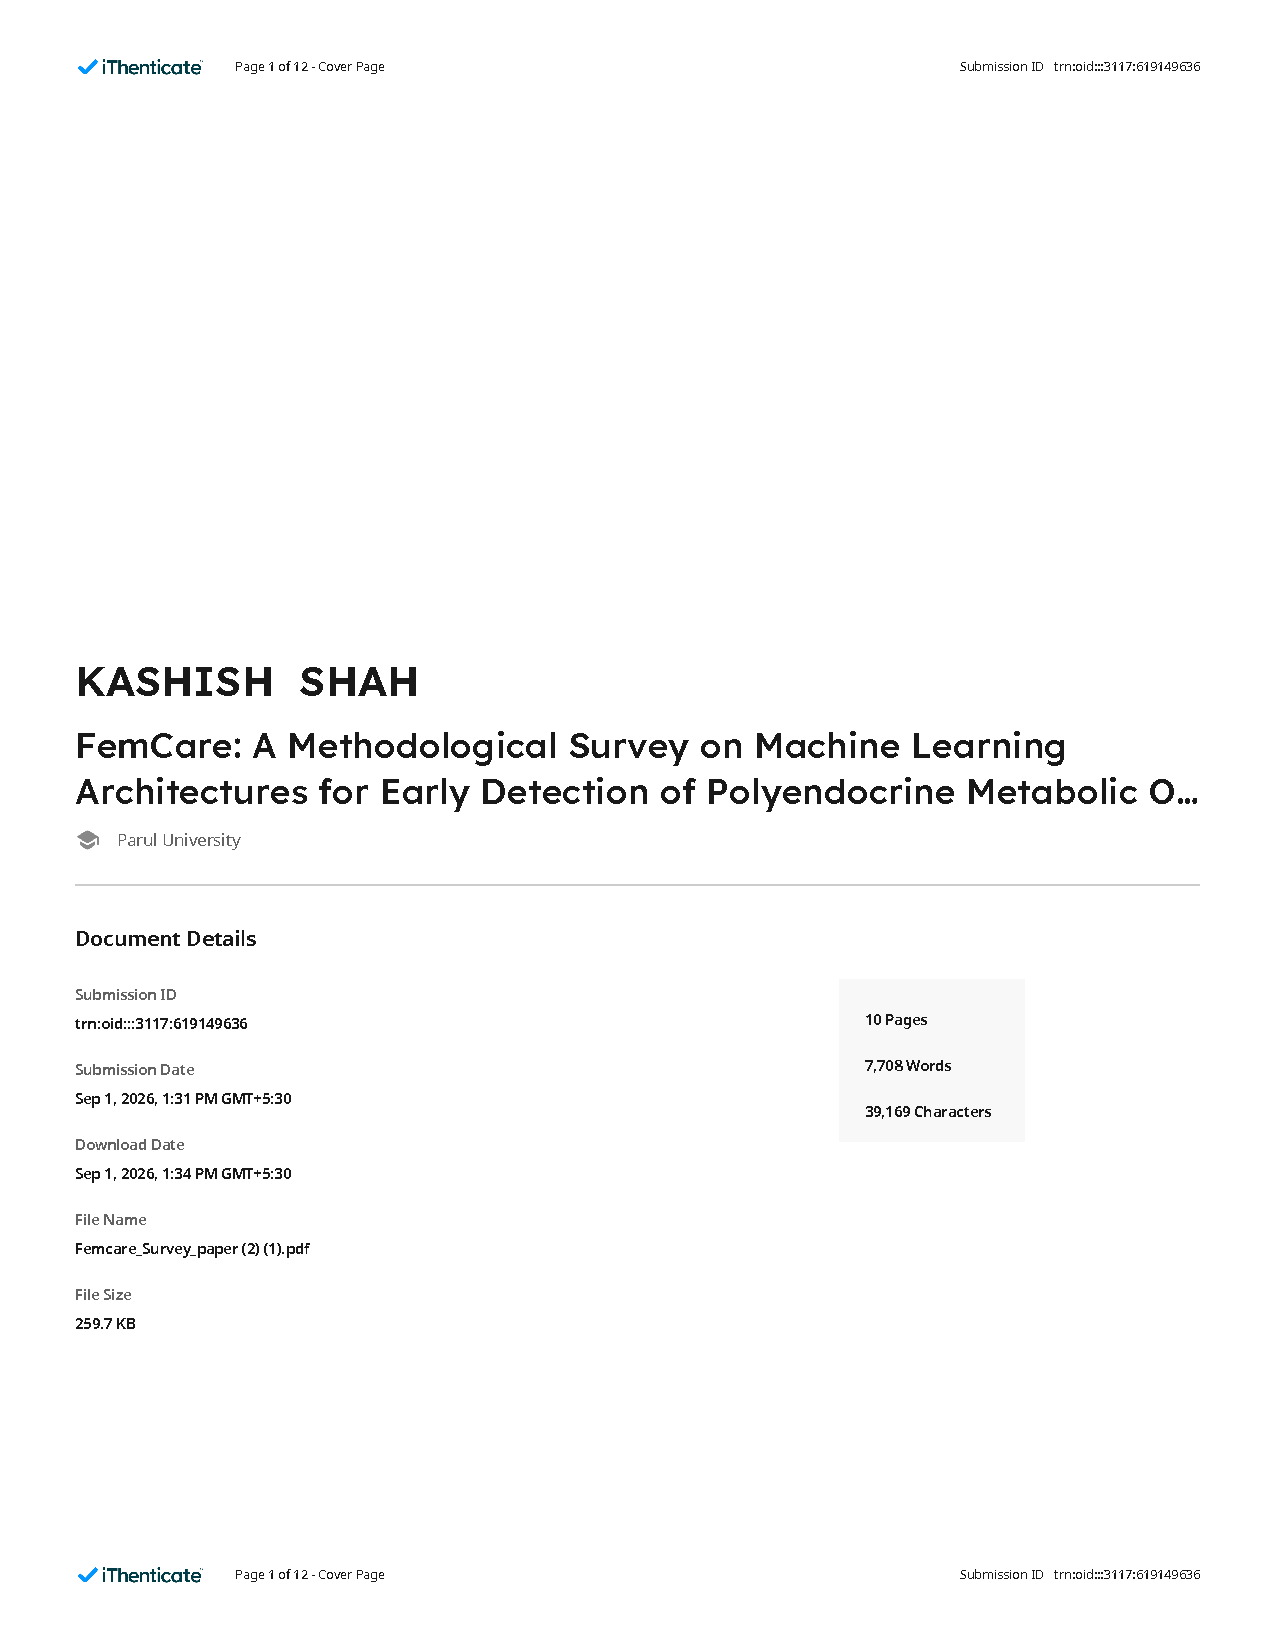
\includepdf[
    pages=-,
    fitpaper=true
]{AIdetection.pdf}

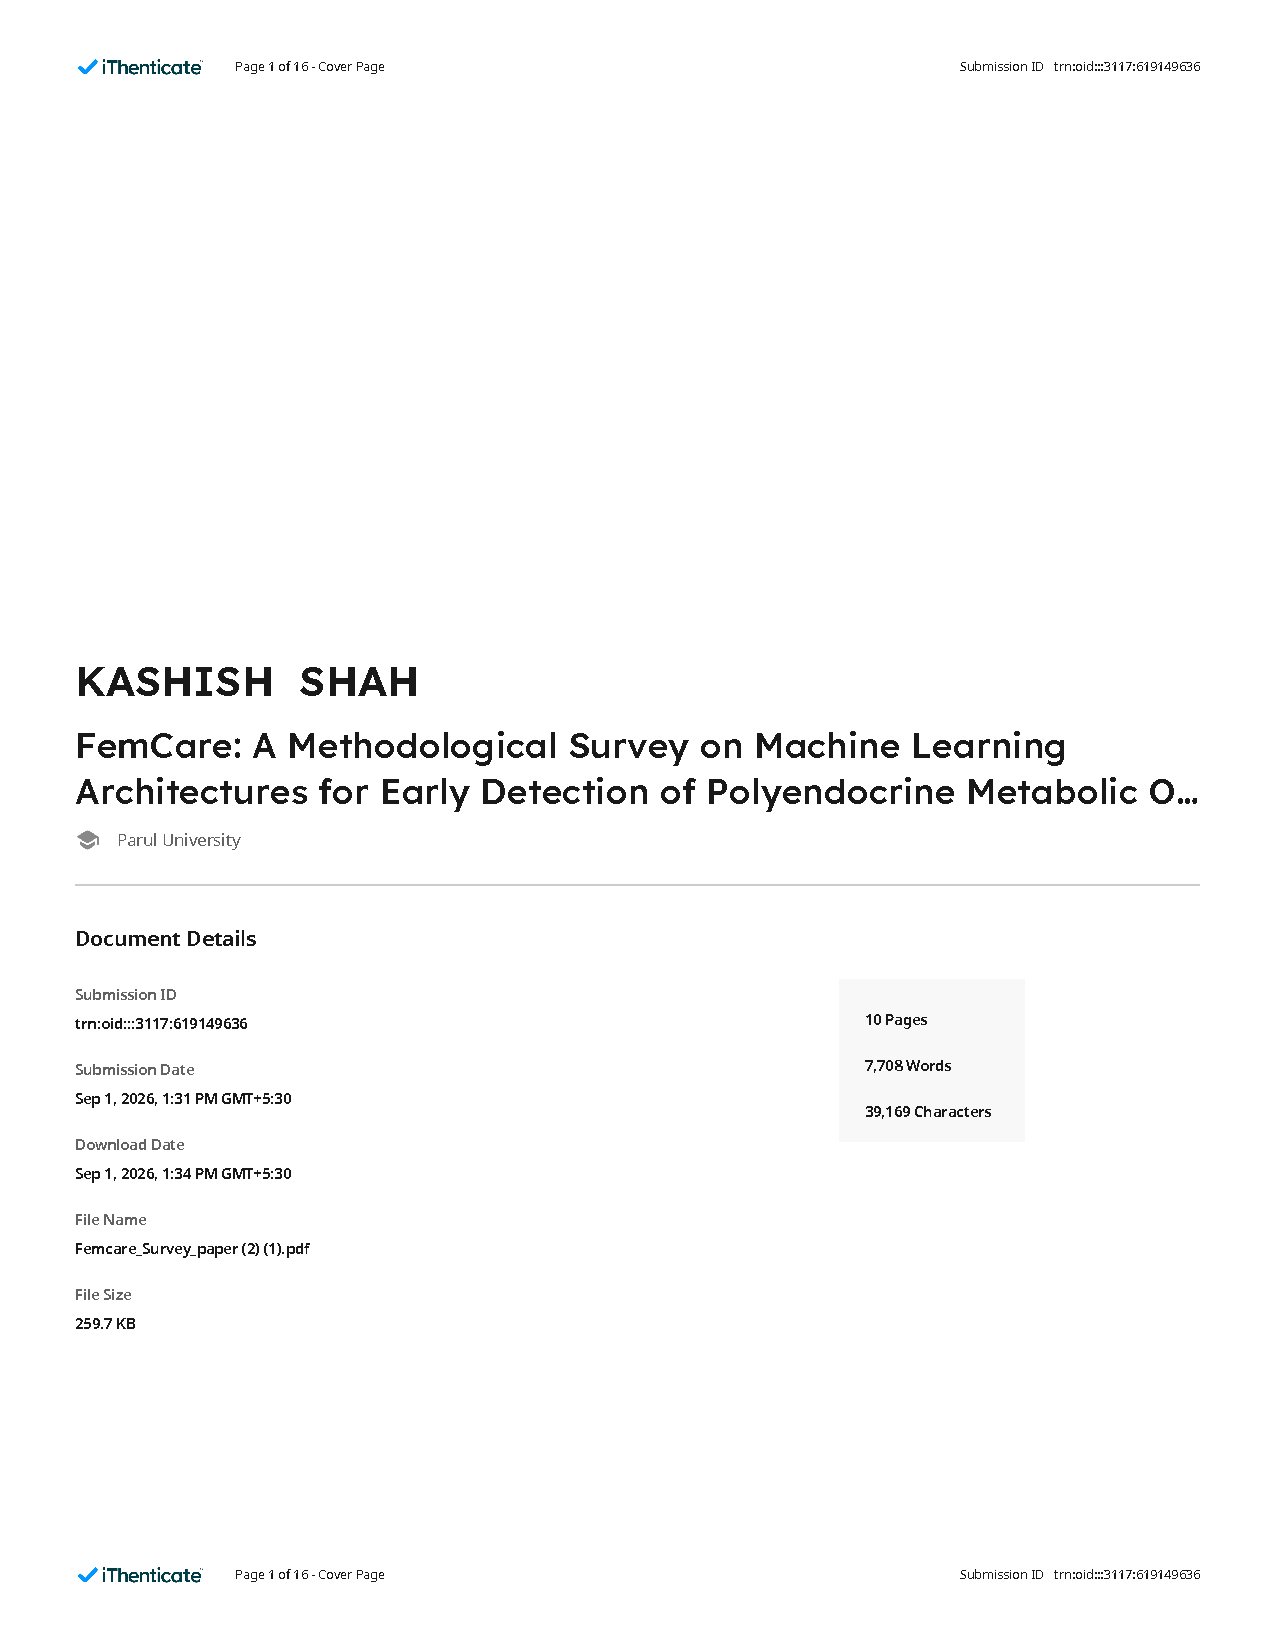
\includepdf[
    pages=-,
    fitpaper=true
]{Plagarism.pdf}


